\documentclass[10pt]{article}
\usepackage{tikz}
\usetikzlibrary{shapes.misc}
\usepackage[margin=0cm]{geometry}
\pagestyle{empty}
\tikzstyle{every node}=[cross out, draw, red]

\begin{document}

\vspace*{\fill}
\begin{center}
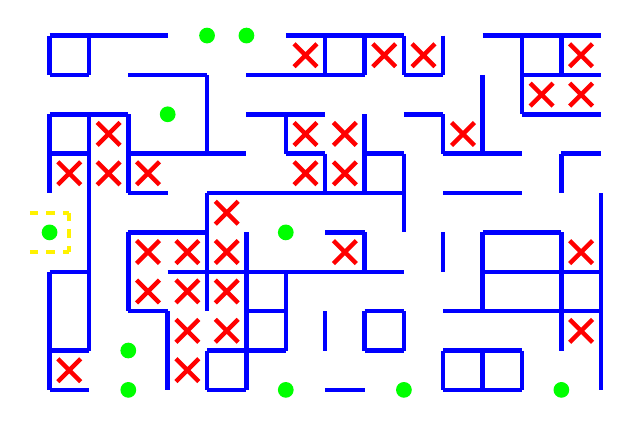
\begin{tikzpicture}[x=0.5cm, y=-0.5cm, ultra thick, blue]
% Walls
    \draw (0,0) -- (3,0);
    \draw (6,0) -- (9,0);
    \draw (11,0) -- (14,0);
    \draw (0,1) -- (1,1);
    \draw (2,1) -- (4,1);
    \draw (5,1) -- (8,1);
    \draw (9,1) -- (10,1);
    \draw (12,1) -- (14,1);
    \draw (0,2) -- (2,2);
    \draw (5,2) -- (7,2);
    \draw (9,2) -- (10,2);
    \draw (12,2) -- (14,2);
    \draw (0,3) -- (1,3);
    \draw (2,3) -- (5,3);
    \draw (6,3) -- (7,3);
    \draw (8,3) -- (9,3);
    \draw (10,3) -- (12,3);
    \draw (13,3) -- (14,3);
    \draw (2,4) -- (3,4);
    \draw (4,4) -- (9,4);
    \draw (10,4) -- (12,4);
    \draw (2,5) -- (4,5);
    \draw (7,5) -- (8,5);
    \draw (11,5) -- (13,5);
    \draw (0,6) -- (1,6);
    \draw (3,6) -- (9,6);
    \draw (11,6) -- (14,6);
    \draw (2,7) -- (3,7);
    \draw (5,7) -- (6,7);
    \draw (8,7) -- (9,7);
    \draw (10,7) -- (14,7);
    \draw (0,8) -- (1,8);
    \draw (4,8) -- (6,8);
    \draw (8,8) -- (9,8);
    \draw (10,8) -- (12,8);
    \draw (0,9) -- (1,9);
    \draw (4,9) -- (5,9);
    \draw (7,9) -- (8,9);
    \draw (10,9) -- (12,9);
    \draw (0,0) -- (0,1);
    \draw (0,2) -- (0,4);
    \draw (0,6) -- (0,9);
    \draw (1,0) -- (1,1);
    \draw (1,2) -- (1,8);
    \draw (2,2) -- (2,4);
    \draw (2,5) -- (2,7);
    \draw (3,7) -- (3,9);
    \draw (4,1) -- (4,3);
    \draw (4,4) -- (4,7);
    \draw (4,8) -- (4,9);
    \draw (5,5) -- (5,9);
    \draw (6,2) -- (6,3);
    \draw (6,6) -- (6,8);
    \draw (7,0) -- (7,1);
    \draw (7,3) -- (7,4);
    \draw (7,7) -- (7,8);
    \draw (8,0) -- (8,1);
    \draw (8,2) -- (8,4);
    \draw (8,5) -- (8,6);
    \draw (8,7) -- (8,8);
    \draw (9,0) -- (9,1);
    \draw (9,3) -- (9,5);
    \draw (9,7) -- (9,8);
    \draw (10,0) -- (10,1);
    \draw (10,2) -- (10,3);
    \draw (10,5) -- (10,6);
    \draw (10,8) -- (10,9);
    \draw (11,1) -- (11,3);
    \draw (11,5) -- (11,7);
    \draw (11,8) -- (11,9);
    \draw (12,0) -- (12,2);
    \draw (12,8) -- (12,9);
    \draw (13,0) -- (13,1);
    \draw (13,3) -- (13,4);
    \draw (13,5) -- (13,8);
    \draw (14,4) -- (14,9);
% Pillars
    \fill[green] (4,0) circle(0.2);
    \fill[green] (5,0) circle(0.2);
    \fill[green] (3,2) circle(0.2);
    \fill[green] (0,5) circle(0.2);
    \fill[green] (6,5) circle(0.2);
    \fill[green] (2,8) circle(0.2);
    \fill[green] (2,9) circle(0.2);
    \fill[green] (6,9) circle(0.2);
    \fill[green] (9,9) circle(0.2);
    \fill[green] (13,9) circle(0.2);
% Inner points in accessible cul-de-sacs
    \node at (6.5,0.5) {};
    \node at (8.5,0.5) {};
    \node at (9.5,0.5) {};
    \node at (13.5,0.5) {};
    \node at (12.5,1.5) {};
    \node at (13.5,1.5) {};
    \node at (1.5,2.5) {};
    \node at (6.5,2.5) {};
    \node at (7.5,2.5) {};
    \node at (10.5,2.5) {};
    \node at (0.5,3.5) {};
    \node at (1.5,3.5) {};
    \node at (2.5,3.5) {};
    \node at (6.5,3.5) {};
    \node at (7.5,3.5) {};
    \node at (4.5,4.5) {};
    \node at (2.5,5.5) {};
    \node at (3.5,5.5) {};
    \node at (4.5,5.5) {};
    \node at (7.5,5.5) {};
    \node at (13.5,5.5) {};
    \node at (2.5,6.5) {};
    \node at (3.5,6.5) {};
    \node at (4.5,6.5) {};
    \node at (3.5,7.5) {};
    \node at (4.5,7.5) {};
    \node at (13.5,7.5) {};
    \node at (0.5,8.5) {};
    \node at (3.5,8.5) {};
% Entry-exit paths without intersections
    \draw[dashed, yellow] (-0.5,4.5) -- (0.5,4.5);
    \draw[dashed, yellow] (-0.5,5.5) -- (0.5,5.5);
    \draw[dashed, yellow] (0.5,4.5) -- (0.5,5.5);
\end{tikzpicture}
\end{center}
\vspace*{\fill}

\end{document}
